\documentclass{standalone}
\usepackage{tikz}
\tikzset{cross/.pic = {  \draw[rotate = 45] (-#1,0) -- (#1,0);
    \draw[rotate = 45] (0,-#1) -- (0, #1);}}
\begin{document}
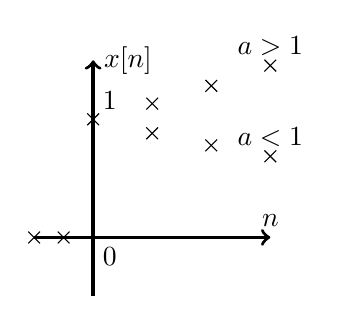
\begin{tikzpicture}[scale=1.5]
    \draw[->,very thick](-0.5,0)--(1.5,0)node[above]{$n$};
        \draw[->,very thick](0,-0.5)--(0,1.5)node[right]{$x[n]$};

        \draw(-0.5,0)pic[black]{cross=3pt};
        \draw(-0.25,0)pic[black]{cross=3pt};
        \draw(0,1)pic[black]{cross=3pt};

        \draw(0.5,1.133)pic[black]{cross=3pt};
        \draw(0.5,0.882)pic[black]{cross=3pt};
        \draw(1,1.284)pic[black]{cross=3pt};
        \draw(1,0.779)pic[black]{cross=3pt};
        \draw(1.5,1.455)pic[black]{cross=3pt};
        \draw(1.5,0.687)pic[black]{cross=3pt};

        \node[above]at(1.5,1.455){$a>1$};
        \node[above]at(1.5,0.687){$a<1$};

        \node[above right]at(0,1){$1$};
        \node[below right]at(0,0){$0$};
\end{tikzpicture}
\end{document}